\chapter{Implementation}
\label{chapter:implementation}

In this chapter we discuss the implementation of the system.
Our main goal is answering the questions posed in \autoref{chapter:introduction}.
In particular --- can we use PoR to solve the integrity problem,
can the reputation system assist in solving this problem,
and how does the validation impact the performance of the network?

In \autoref{chapter:analysis} we discussed how the system would work in an ideal world,
and in this chapter we discuss how we have implemented the system ---
what shortcuts we have taken, what trade-offs we have made,
how do they affect the system, and what we have learned from the implementation.

While answering the research questions is our main goal,
we also want to design the system with the best software practices in mind.

\section{Architecture}

The overall architecture has not changed much from the prior work.
We have added a new module responsible for simulating malicious peer behavior,
which uses the local storage in order to tamper with the files.
The other modules have seen some refactoring and new additions,
but the core architecture remains the same.
The architecture of the system is shown in \autoref{fig:architecture}.

\begin{figure}
    \centering
    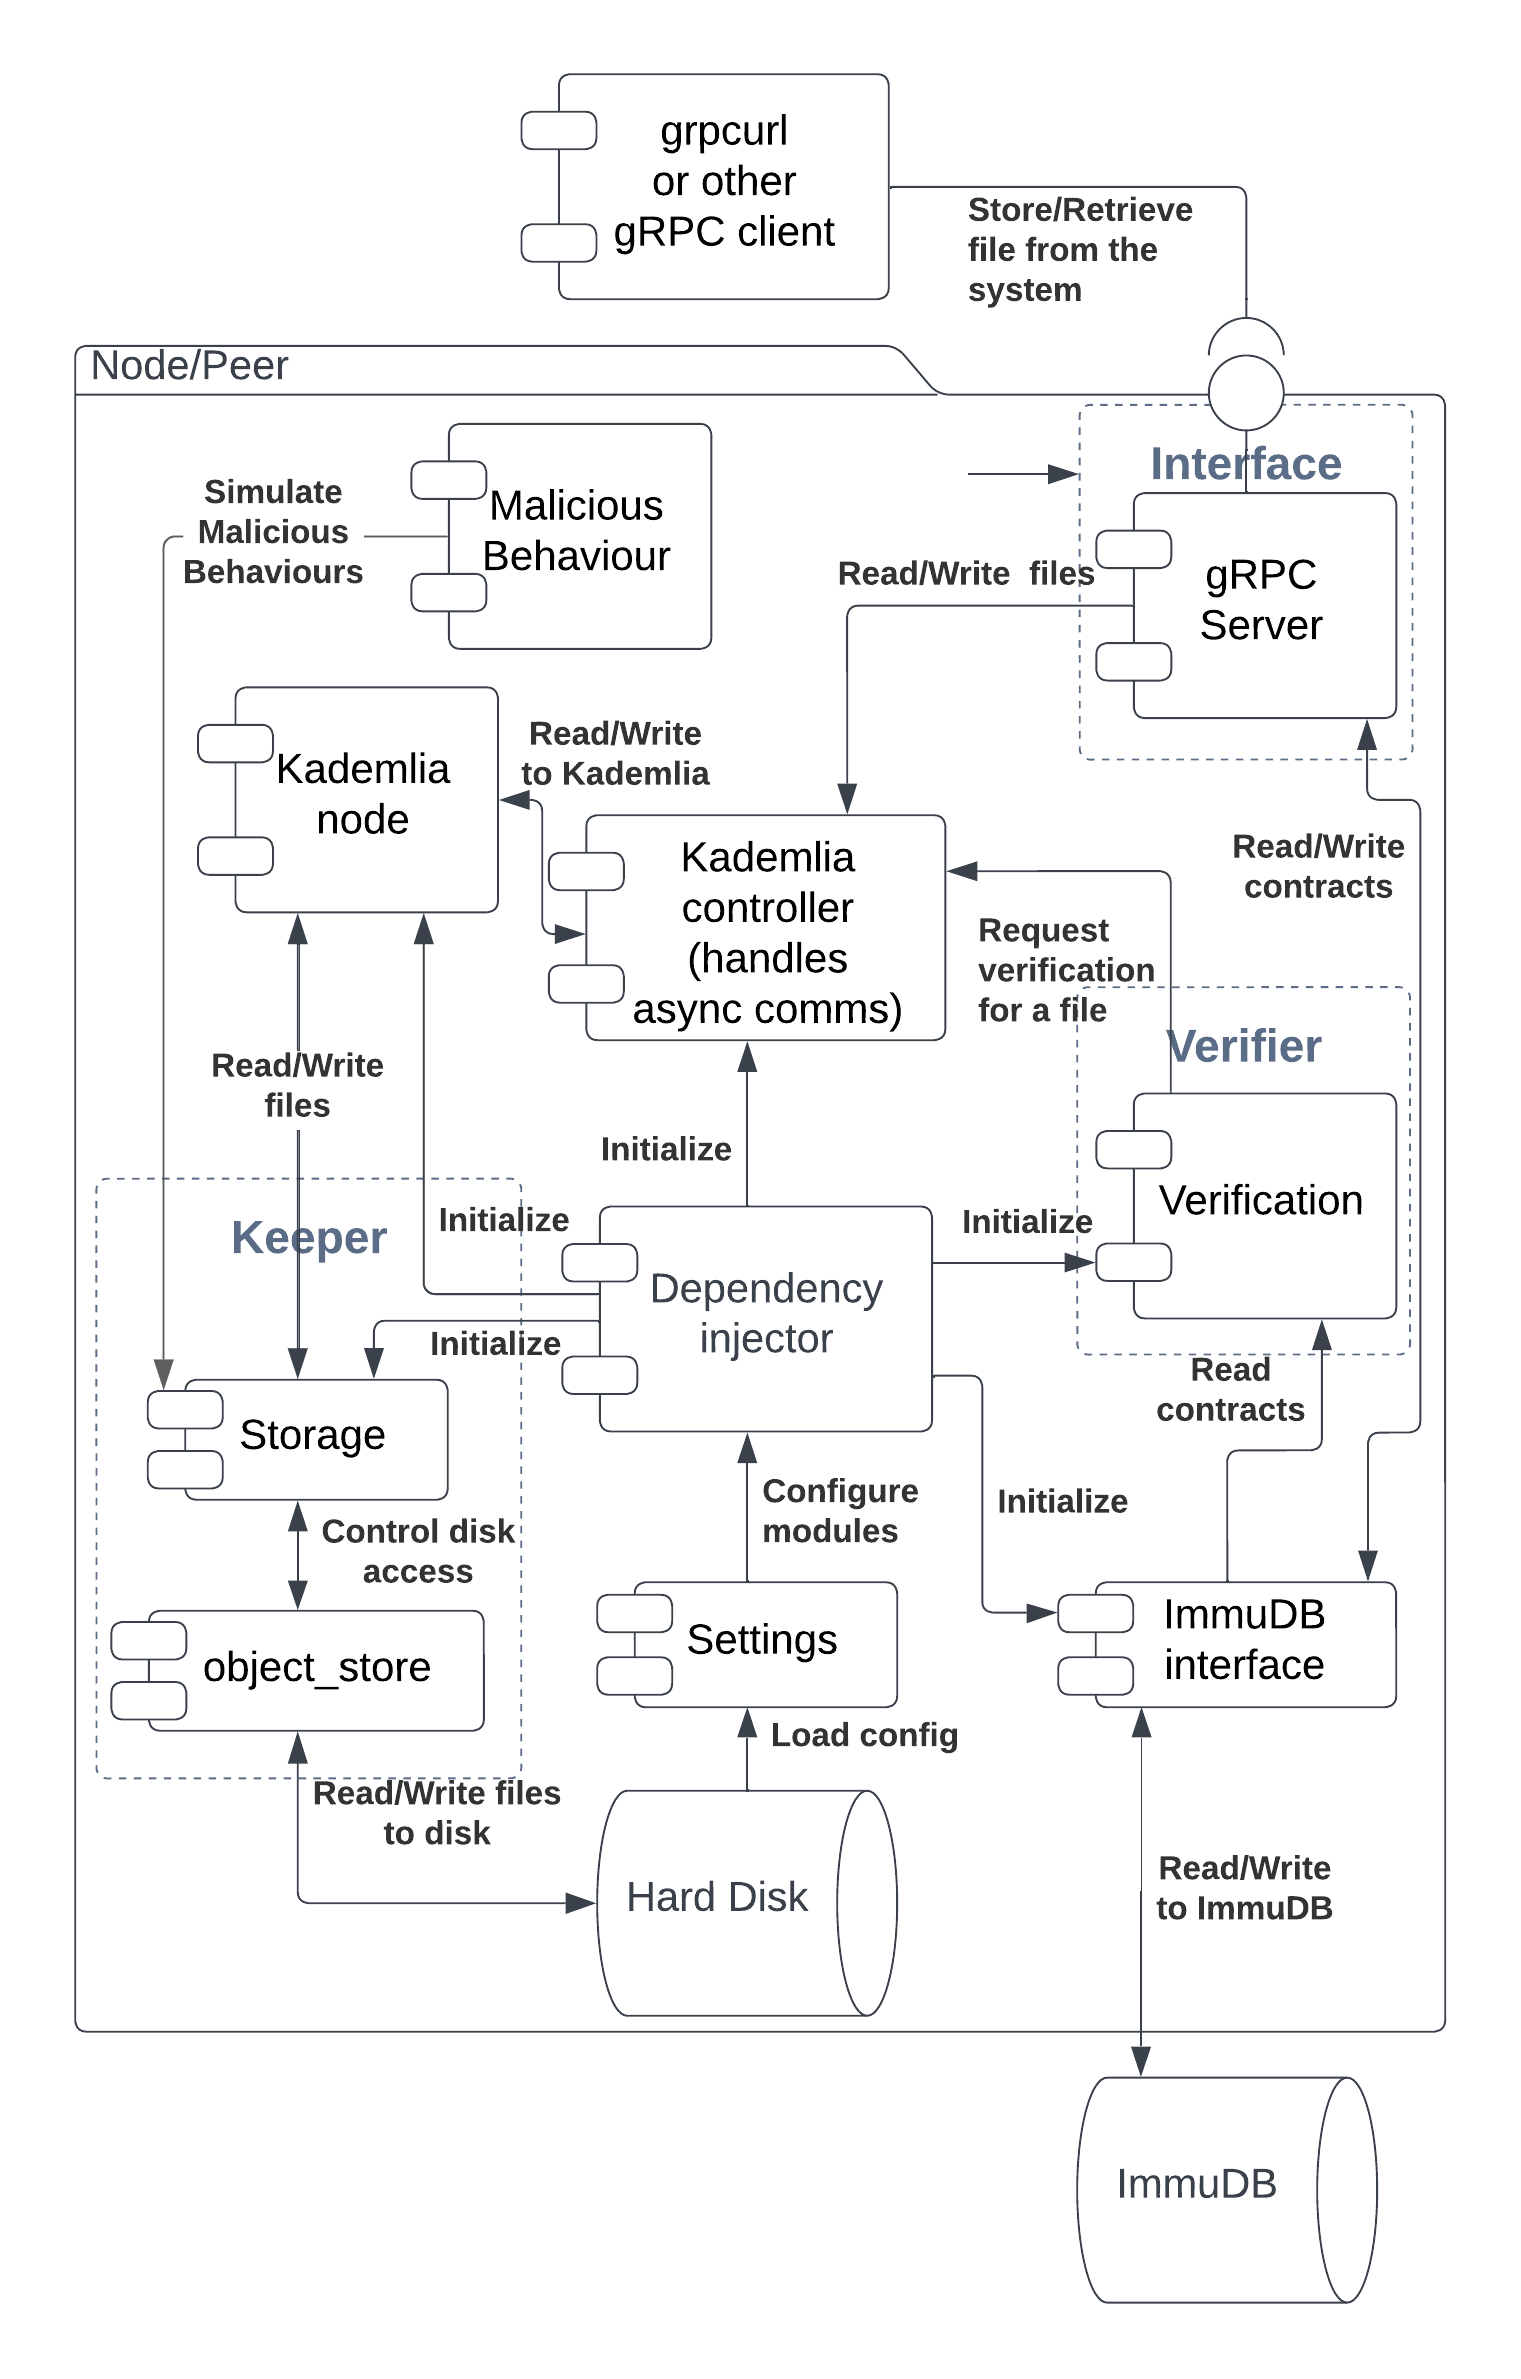
\includegraphics[width=1\textwidth]{gfx/architecture.png}
    \caption{Updated architecture of the system}
    \label{fig:architecture}
\end{figure}

\section{Modules and dependency injection}

The architecture of the system revolves around dynamically loading modules.
We want to easily exchange the different implementations of the components in the system.
For example, we want to change the storage layer from local storage to a Docker container,
or for testing we want to quickly change the behavior of peers --- whether it is malicious or not.

To achieve this we make use of the \texttt{config} crate to load the configuration.
Configuration is hierarchical and is loaded from multiple sources.
First we load the base configuration from a \texttt{.yaml} file.
Then we load an optional configuration \texttt{.yaml} file that can override the base configuration.
Finally, we load any environment variables that can override the configuration.
In \autoref{lst:config} we show an example of a partial configuration file.
We need partial configuration files because during testing we want to start each peer on a different port.
It is useful to be able to change the \texttt{grpc.port} field or to be able to pass it as an
environment variable \texttt{GRPC\_PORT} because a lot of our end-to-end tests are bash scripts,
which start hundreds of peers in parallel.

\begin{lstlisting}[caption={Example of a configuration file}, label={lst:config}]
storage:
  type: local
  path: data/peer1
grpc:
  port: 2000
malicious_behavior:
  type: none
\end{lstlisting}

Once the configuration is loaded we pass it to the dependency injector,
for which we use the crate \texttt{runtime\_injector}.
It reads the configuration and instantiates the different modules based on it.
For example when we initiate the malice, inject the implementation of the storage module
and based on the settings in the configuration, we initialize a different malicious behavior,
i.e., we provide a different implementation for the malice module.
An example of how this works can be seen in \autoref{lst:injector}.

\begin{lstlisting}[language=Rust, style=colouredRust, caption={Example of dynamically loading a module}, label={lst:injector}]
let settings = injector.get::<Svc<dyn ISettings>>()?.malicious_behavior();
let storage = injector.get::<Svc<dyn IStorage>>()?;

match settings {
    MaliciousBehavior::None =>
        Ok(Box::<MaliceNone>::default()),
    MaliciousBehavior::DeleteAll =>
        Ok(Box::new(MaliceDeleteAll::new(storage))),
    MaliciousBehavior::DeleteRandom(_) =>
        Ok(Box::new(<MaliceDeleteRandom>::new(storage))),
}
\end{lstlisting}

The dependency injector in combination with the configuration is a powerful tool,
as it allows us to easily change the behavior of the system, without making code changes.
It also allows us to develop the system in a modular way,
where each module is independent of the others, and only depends on the interfaces of the other modules.
The dependency injection crate handles converting each module to a singleton service,
passing a reference to that service to the other modules that depend on it,
and resolving the dependency graph.
The one thing it does not handle is the case when each module runs in a different thread,
and we need to ensure that the modules are thread safe.
In this case we have to manually enclose the modules in a Mutex,
which is not ideal, but it is a trade-off we are willing to make for the flexibility of the system.

\section{Ledger}

The only component in the system we have implemented that is not distributed is the ledger.
The ledger acts as the catalog for the files stored in the network,
as well as the reputation of the peers.
Ideally the ledger should be distributed in order for the system to be fully decentralized.
An example of a distributed ledger technology is any blockchain.
Initially we considered using one of Near, Solana, or Substrate \cite{near, solana, substrate}.
These are all blockchains implemented in Rust, which is the language we are using for the implementation.
This would have allowed us to easily integrate the ledger more easily with the rest of the system.
However, we decided against using a blockchain for the ledger for this implementation
mainly because of the complexity of integrating with a blockchain.
We see this as a future work in order to make the system production ready,
and we discuss the integration with a blockchain in the \autoref{chapter:future-work}.

\section{Using the immutable database Immudb}
\label{section:using-immudb}

The backbone of the integrity of the system is the immutable database Immudb \cite{immudb}.
An immutable database ensures we can store the metadata necessary to run the system
in a tamper-proof way.
The database acts as a form of catalog for the files stored in the network,
storing the keys and metadata required to perform audits.
Immudb is a lightweight, high-speed immutable database that is designed to be used as a key-value store.
It is based on the Merkle tree data structure, which allows for efficient verification of the integrity of the data.
The database is designed to be tamper-proof, meaning that although the database supports updates and deletes,
the history of the data is always preserved.
If a record is changed or deleted,
the database keeps a record of the change, and the history of the record can be traced back to its creation.
This property is crucial for the reputation system, as it ensures that the reputation scores are not tampered with,
or if they are tampered with the client of the database can detect the tampering.

\subsection{Using Immudb at scale}

One downside of the database is that it is not innately designed to be distributed.
This means that the database is not designed to be run on multiple nodes,
and it does not support replication out of the box.
In a real-world scenario, running the database on a single node is a huge flaw,
as it makes the database a single point of failure.
For the purposes of our experiments, we run the database on a single node.
However, we will briefly discuss how the database can be made distributed in the future.
The first approach is by distributing the Immudb itself.
We could shard the data and run multiple instances of the database on different peers.
Since the database is immutable, peers can be sure that the data is consistent across all the nodes.
For example, sharding the data could be done by taking the file key, or the hash of the file key as the shard key.
This way it would be easy to locate where the metadata for a given file is stored.
The second approach is to use the storage system itself, completely removing the need for the database.
This would require more work to ensure the system can support the same operations as the database,
but it would simplify the querying, as the metadata would be stored in the same place as the files.

\subsection{Atomic Operations in Immudb}
\label{section:atomic-operations}

The second downside of the database is that it does not support complex queries.

For example, we need to atomically update the reputation of a peer after a successful audit.
Since audits may happen in parallel, we need to ensure that the reputation is updated correctly.
This means that we need to read the current reputation of the peer, increment it, and write it back to the database.
This operation needs to be atomic, as we do not want to lose any updates.

\begin{lstlisting}[language=SQL, caption={SQL query to update the reputation of a peer}, label={lst:sql-query}]
BEGIN TRANSACTION;
DECLARE @value INT;
SELECT @value = reputation FROM reputations WHERE peer_id = @peer_id;
UPDATE reputations SET reputation = @value + 1 WHERE peer_id = @peer_id;
COMMIT TRANSACTION;
\end{lstlisting}

The above query would work in a traditional SQL database, but it would not work in Immudb,
because Immudb supports only simple SELECT, INSERT, UPDATE, and DELETE operations.
Luckily it does support transactions, which we can use to ensure that the operation is atomic.

Immudb supports two ways of authentication, both making use of a token.
The first way is to log in as a temporary user, which enables the use of single SQL queries.
For example, after a login, we can execute an INSERT followed by a SELECT followed by another INSERT.
These queries are independent of each other.
If we want to use transactions, we need to log in and establish a session, followed by initiating a transaction.
These two operations return unique tokens that we need to pass as headers with each subsequent request.
Initiating a transaction is the equivalent of the SQL BEGIN TRANSACTION command.
This way, the database knows which session and transaction we are referring to.
The session token is used to authenticate the user,
while the transaction token is used to ensure that the operations are atomic.
After we execute the operations, we need to commit the transaction to make the changes permanent.
Lastly we need to close the session to free up resources.

\subsection{Conflict Resolution}

Immudb does not support conflict resolution out of the box.
Under the hood, immudb uses transactions even in the case of a non-session login.
The delay in the transactions is minimal, but it can affect the queries.
In particular, if two writes happen at the same time (or close to each other),
the database returns an error --- \texttt{ErrTxReadConflict}.
This error stands for "tx read conflict" and it means that the transaction was not successful
because another transaction was committed in the meantime.
It occurs even when the query is not a transaction,
so for example when adding a new file to the database, and we write the contract to the database, it can fail.
Immudb does not provide a way to automatically retry the transaction,
so we had to implement the retry mechanism in the client.
The official documentation acknowledges this issue and mentions that MVCC (Multi-Version Concurrency Control)
is on the roadmap, but not yet implemented, hence such failures are expected and need to be handled by the client.

\subsection{Using Immudb to store the files (rejected idea)}

One way for us to verify that a malicious peer is not modifying/deleting the files is
to store the files in an immutable database (this does nothing against bit rot or hardware failures).
Since it is immutable, it preserves the history of the data, and we can always request to see the history
of the file to verify that it has not been tampered with.
So why do we not run an Immudb instance on each peer and store the files in it?
The reason is that this introduces additional complexity.

While the peer cannot modify the file, without leaving a trace,
it can always wipe the database and recreate it.
This erases the history and make it seem like no changes were made.
Any data stored on the peer is at risk of being deleted or modified,
and therefore cannot be trusted.
Perhaps we can check the timestamp of the time of storing the file,
but this can be easily modified by the peer if they use a modified Immudb instance.

These and more considerations would need to be made if we were to use this approach.
It enables a different class of attacks for which we would need to augment the system.
In particular, we would need to implement ways to deal with these attacks in the Kademlia layer,
and we would need to implement a new storage interface for Immudb, that Kademlia can use.

While this is not impossible, it is considerably more work than adapting Kademlia to
work with PoR and store files on the disk.

\section{Kademlia}

Kademlia is the distributed hash table (DHT) that we use to store the files in the network.
We are using the implementation from the official Rust libp2p crate \cite{rustlibp2p}.
We have made some extensions to the implementation to support our use cases.
One of these is the local storage, which we touch upon in the following section.
We have also included a direct peer to peer communication channel,
which is referred to as a request-response protocol in the libp2p documentation,
and we use it to perform audits required for the Proof of Retrievability.
This was required since the base implementation of Kademlia is closed for extension,
and we needed a way to communicate with the peers directly.

An important note here is that the Kademlia implementation supports only some basic operations,
some of which differ from the original Kademlia paper.
For example, the storage operation stores the value on the current node,
while the original Kademlia paper stores the value on the closest node to the key.
Therefore, to achieve the original behavior of the Kademlia paper,
we had to implement part of the Kademlia protocol ourselves.
For the PUT operation in particular, we first use GET\_CLOSEST\_PEERS to find the closest peers to the key,
and then perform the PUT operation on the peers we found.
This was not a huge downside since it allowed us to easily inject the PoR protocol into this operation.
The initialization step of the PoR protocol happens when we store the file for the first time.
We have to create a secret vector that the Keeper, where the file is stored, does not know.
So once we find the closest peers to the key, we initialize the PoR secret vector,
and then we store the file on the Keeper,
while simultaneously storing the PoR secret as well as additional metadata in the ledger.

\section{Local Storage}

We rely on Kademlia to store files in the network.
Or more precisely, we rely on the Kademlia protocol to route the files to the correct peer.
However, the implementation of the Kademlia protocol in
the \texttt{libp2p} crate does not support storing the files on the disk.
It only comes with a simple in-memory storage, designed for testing and examples.

Since we want the storage to be persistent, we need to implement our own storage module.
Fortunately, the \texttt{libp2p} crate is designed to be easily extensible.
It provides a storage interface that we can implement to store the files on the disk.
The implementation can be split into two parts --- converting the Record to bytes
and storing the bytes to disk.

Files in Kademlia are shared as Records.
A Record is the key, value, publishers, and expiration date.
We cannot store only the value, because when the file is requested,
it is requested as a Record, and we need to reconstruct the Record.
If we are missing the metadata, we cannot construct a valid Record.
Unfortunately, serializing and deserializing a Record is not trivial.
The Record is not designed to be serializable, mainly due to the expiration date field.
The expiration date is a Duration, which is a struct intended for internal use in code.
It supports very precise time calculations, additions, and comparisons,
but it is not designed to be sent over the network or serialized.
Sending the Duration over the network is not an issue for us,
since we do not need nanosecond precision for the expiration date.

We implemented a custom serializer for the Record,
which serializes the Record to bytes in a YAML format.
Record is a struct from the \texttt{libp2p} crate,
and therefore we cannot change it or extend it by implementing serialization for it.
However, we can use a workaround --- we can create a wrapper struct around the Record,
and implement all the necessary functionality for it.
A wrapper struct is not ideal, since we cannot break the scope of the Record fields,
i.e., we cannot access the private fields of the Record.
But with using the getter/setter methods, we can access the fields of the Record,
and implement the serialization and deserialization.

The second part of the storage module is writing or reading the bytes to or from the disk.
To achieve this we use the crate \texttt{object\_store}, which provides
asynchronous file operations using an S3-like interface.
The choice of using an S3-like interface is guided by the fact that a lot of
storage solutions provide an S3-compatible interface.
These range from cloud storage, to local disk storage (as this crate), to storage apps
running in Docker containers.
This essentially means that, we can easily isolate the stored files from the rest of the system,
by running a Docker container and connecting to it using the S3 interface.
This is a huge advantage, as it allows us to not worry about what files are being stored.
Even if a malicious file is stored, it is isolated from the rest of the system,
and it cannot affect the rest of the system.

Having asynchronous file operations is a good feature as they do not block the rest of the system,
and file operations can be slow.
Kademlia's interface, however, is synchronous, and we need to adapt the asynchronous file operations.
We achieve this by spawning a new thread for the file operation and blocking
until the operation is finished.
This is a workaround that prevents parallel file operations,
but it does not block the whole system, since Kademlia is running in a separate thread.

Implementing the storage module is a big step towards making the system production ready.
It also helps immensely in testing, as we can easily inspect the files stored on the disk,
and rerun benchmarks without having to initialize the state of the system every time.

\section{Malicious Peer Behaviors}

When we talk about malicious behaviors in the network,
we are not necessarily interested whether they are intended or not.
Corrupting a file could be both intentional and unintentional,
and both cases can be implemented in the same way.
We will refer to these behaviors as malicious behaviors.

In order to test the system, we need to simulate malicious peer behaviors.
We have implemented a few malicious peer behaviors that we use to test the system.
These behaviors get injected as a module into the peer,
and they can be turned on or off at any time.
The dependency injector is a huge help here, as we can easily change the behavior of the peer
by changing the configuration file.

All behaviors are implemented similarly to each other.
They run an infinite loop, that triggers every few seconds.
Inside the loop they perform a malicious action.
For example, the behavior that does not store any files,
checks if any new files have been stored on the peer, and deletes them.

\section{gRPC Gateway}

Interacting with the system is done through the gRPC gateway.
gRPC is a high-performance, open-source universal RPC framework.
It is designed to be efficient and lightweight, and it is based on HTTP/2.
For our purposes these are nice to have features but not crucial,
because we use gRPC only for the communication between the client and the first peer.
For example, if we want to upload a file to the network,
we send a request to upload a file with the file's contents to one peer over gRPC.
Since clients usually run their own peer, this communication is local,
and therefore very fast, regardless of the protocol used.

We chose gRPC because it is widely adopted and has good support in the face of
tools and libraries.
Also, in an earlier version of the system, we used gRPC to communicate between the peers,
in particular the verification was done over gRPC.
We have since moved the verification to the Kademlia layer,
but we kept the gRPC gateway for the client to communicate with the first peer.

To implement gRPC we define the interfaces in a \texttt{.proto} file,
and then we use the \texttt{tonic} crate to generate the server and client code.
The \texttt{tonic} crate is a gRPC implementation for Rust,
that generates the boilerplate code of running a gRPC server and client for us.
To implement the server we simply implement the generated interfaces
and provide the implementation to the server.

An example of a \texttt{.proto} definition could be \autoref{lst:proto}.

\begin{lstlisting}[caption={Example of a .proto file}, label={lst:proto}]
message RetrieveRequest {
    string name = 1;
}

message RetrieveResponse {
    bytes content = 2;
}

service KissService {
    rpc Store(StoreRequest) returns (StoreResponse);
}
\end{lstlisting}

This definition defines a service called \texttt{KissService} with one method \texttt{Retrieve},
that we can then implement in Rust such as \autoref{lst:grpc-server}.

\begin{lstlisting}[caption={Example of a gRPC server implementation}, label={lst:grpc-server}, language=Rust, style=colouredRust]
impl KissService for KissServiceImplementation {
    async fn retrieve(
        &self,
        request: Request<RetrieveRequest>,
    ) -> Result<Response<RetrieveResponse>, Status> {
        // ... get file from Kademlia

        Ok(Response::new(RetrieveResponse {
            file_content,
        }))
    }

\end{lstlisting}

Once we have the server implemented, we tell \texttt{tonic} to run the server,
and handle requests by calling the methods of \texttt{KissServiceImplementation}.

Calling the peer is now as simple as sending a gRPC request with a tool like \texttt{grpcurl} \autoref{lst:grpc-request}.

\begin{lstlisting}[language=bash, caption={Example of a gRPC request}, label={lst:grpc-request}]
    grpcurl \
    -plaintext \
    -import-path proto \
    -proto kiss.proto \
    -d "{\"name\": \"<OUR-FILE-UUID>\"}" \
    '[::1]:2000' \
    kiss_grpc.KissService/Retrieve
\end{lstlisting}

In \autoref{fig:store} we can see the sequence of operations that happen
when we store a file in the network through the gRPC gateway.

\begin{figure}
    \centering
    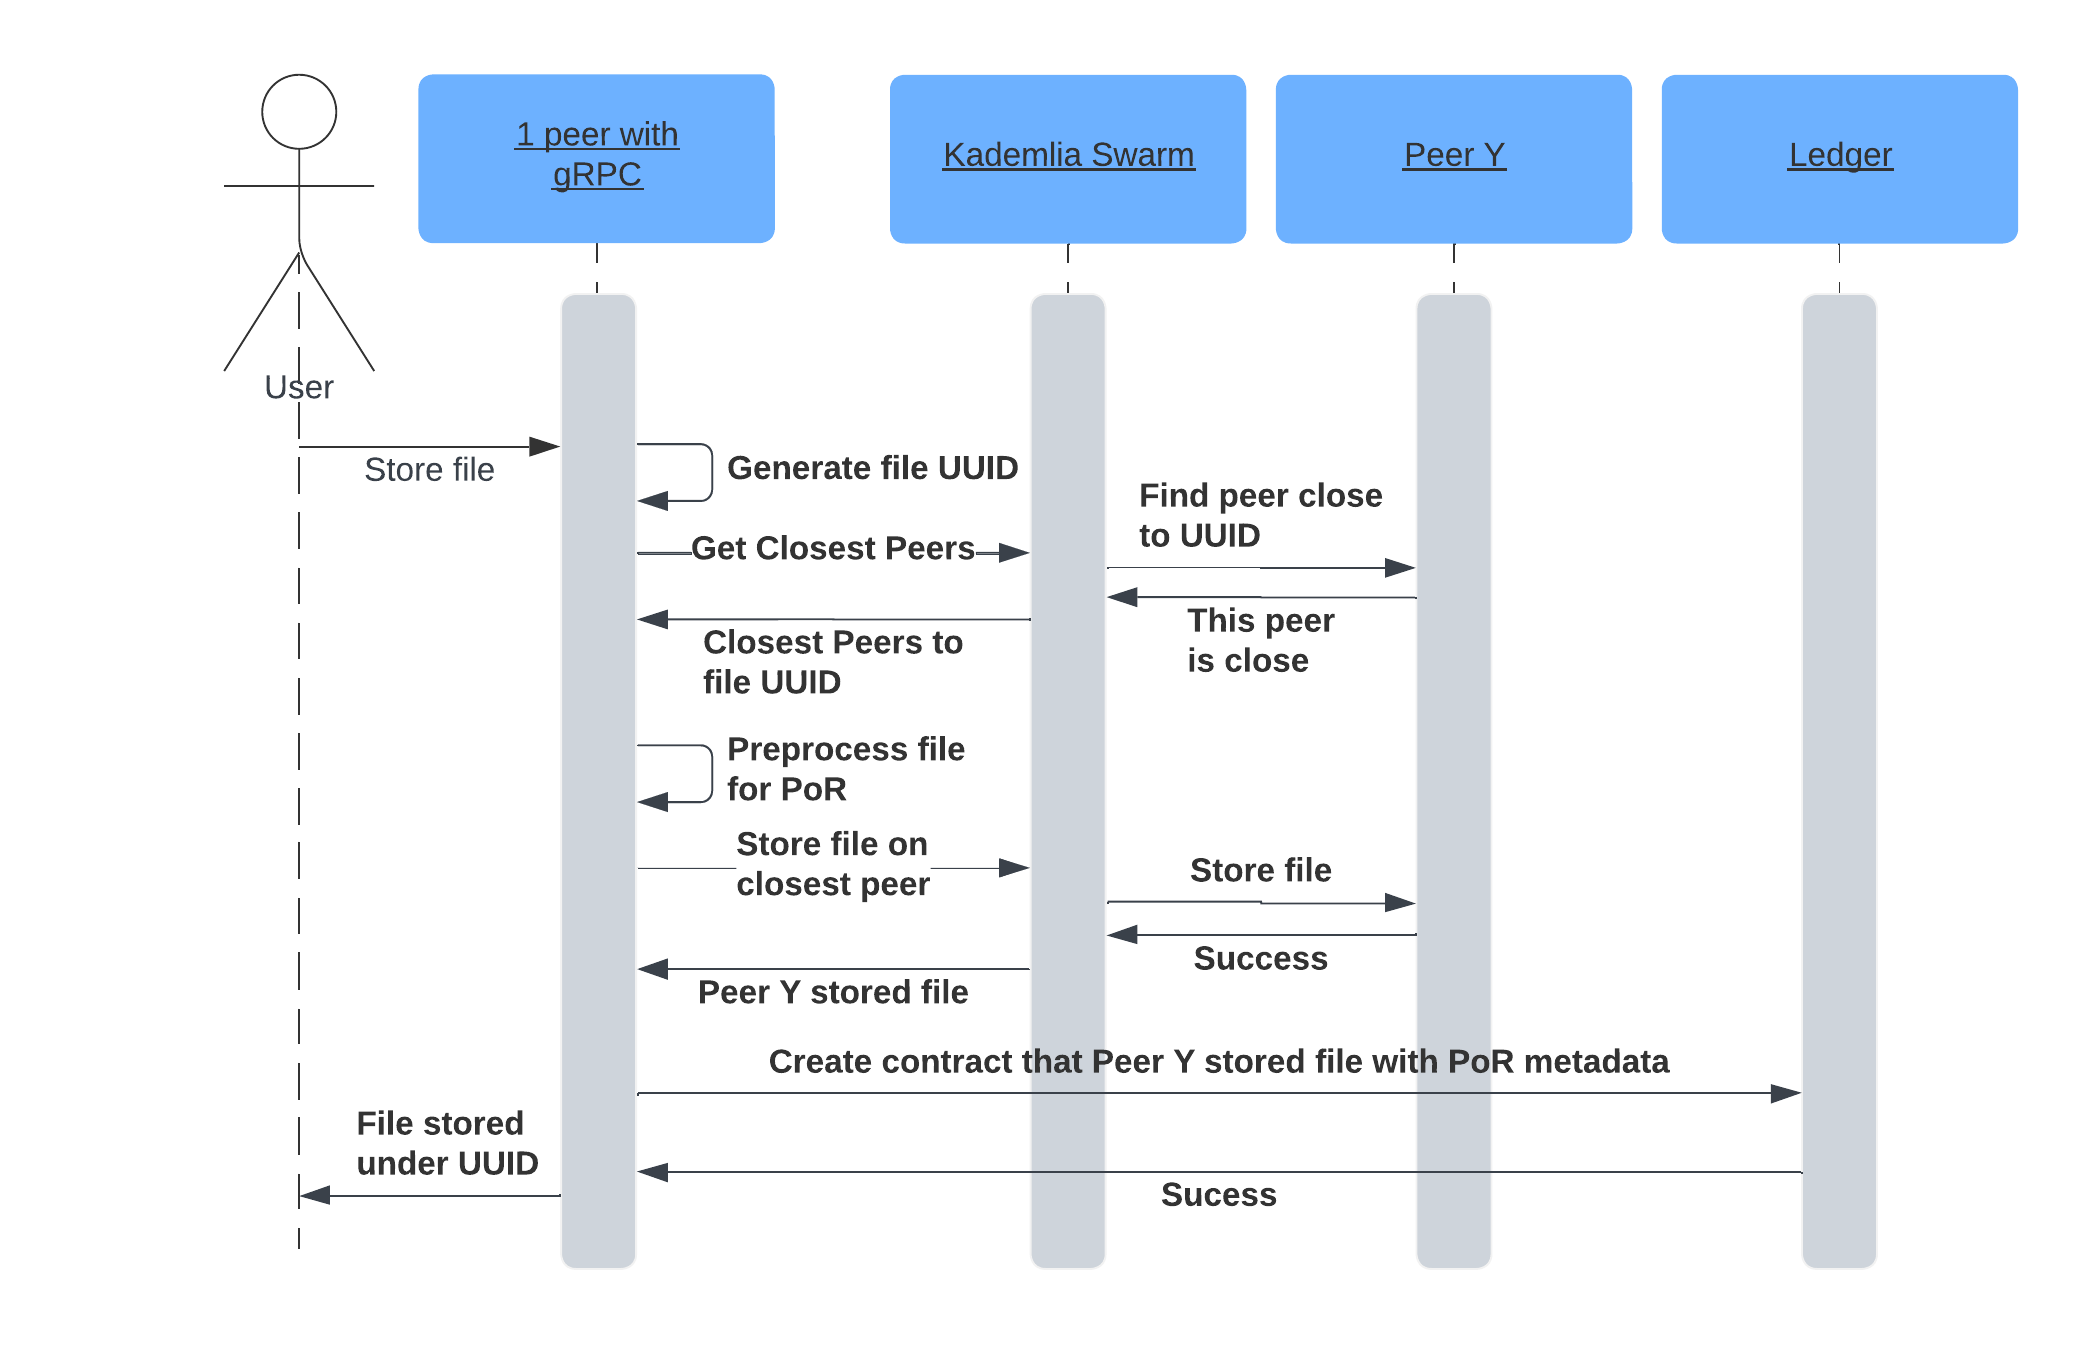
\includegraphics[width=1\textwidth]{gfx/store.png}
    \caption{Storing a file in the network}
    \label{fig:store}
\end{figure}

An important note is that by default the gRPC crate, \texttt{tonic},
processes requests with maximum size of 4MB.
We need to increase this size by setting the \texttt{max\_decoding\_message\_size} and
\texttt{max\_encoding\_message\_size} in the gRPC configuration to a higher value.
Similarly, in the Kademlia module we have to set the \texttt{set\_max\_packet\_size}
to a higher value, because by default Kademlia does not allow sending packages larger than 1MB.

We have chosen to use an external tool to make the requests,
instead of implementing a client, because it allows faster iteration and testing.
If the server changes we do not need to recompile the client,
or change the names of the endpoints in the client.
For testing purposes, UNIX provides plenty of tools that can record network traffic,
time the requests, and so on, so it is easier to use them than to implement a client.

\section{Proof of Retrievability}

We run the PoR protocol during each verification of a file.
The protocol has two steps --- the Verifier generates a challenge and
the Keeper responds to the challenge, as seen in \autoref{fig:verify}.

\begin{figure}
    \centering
    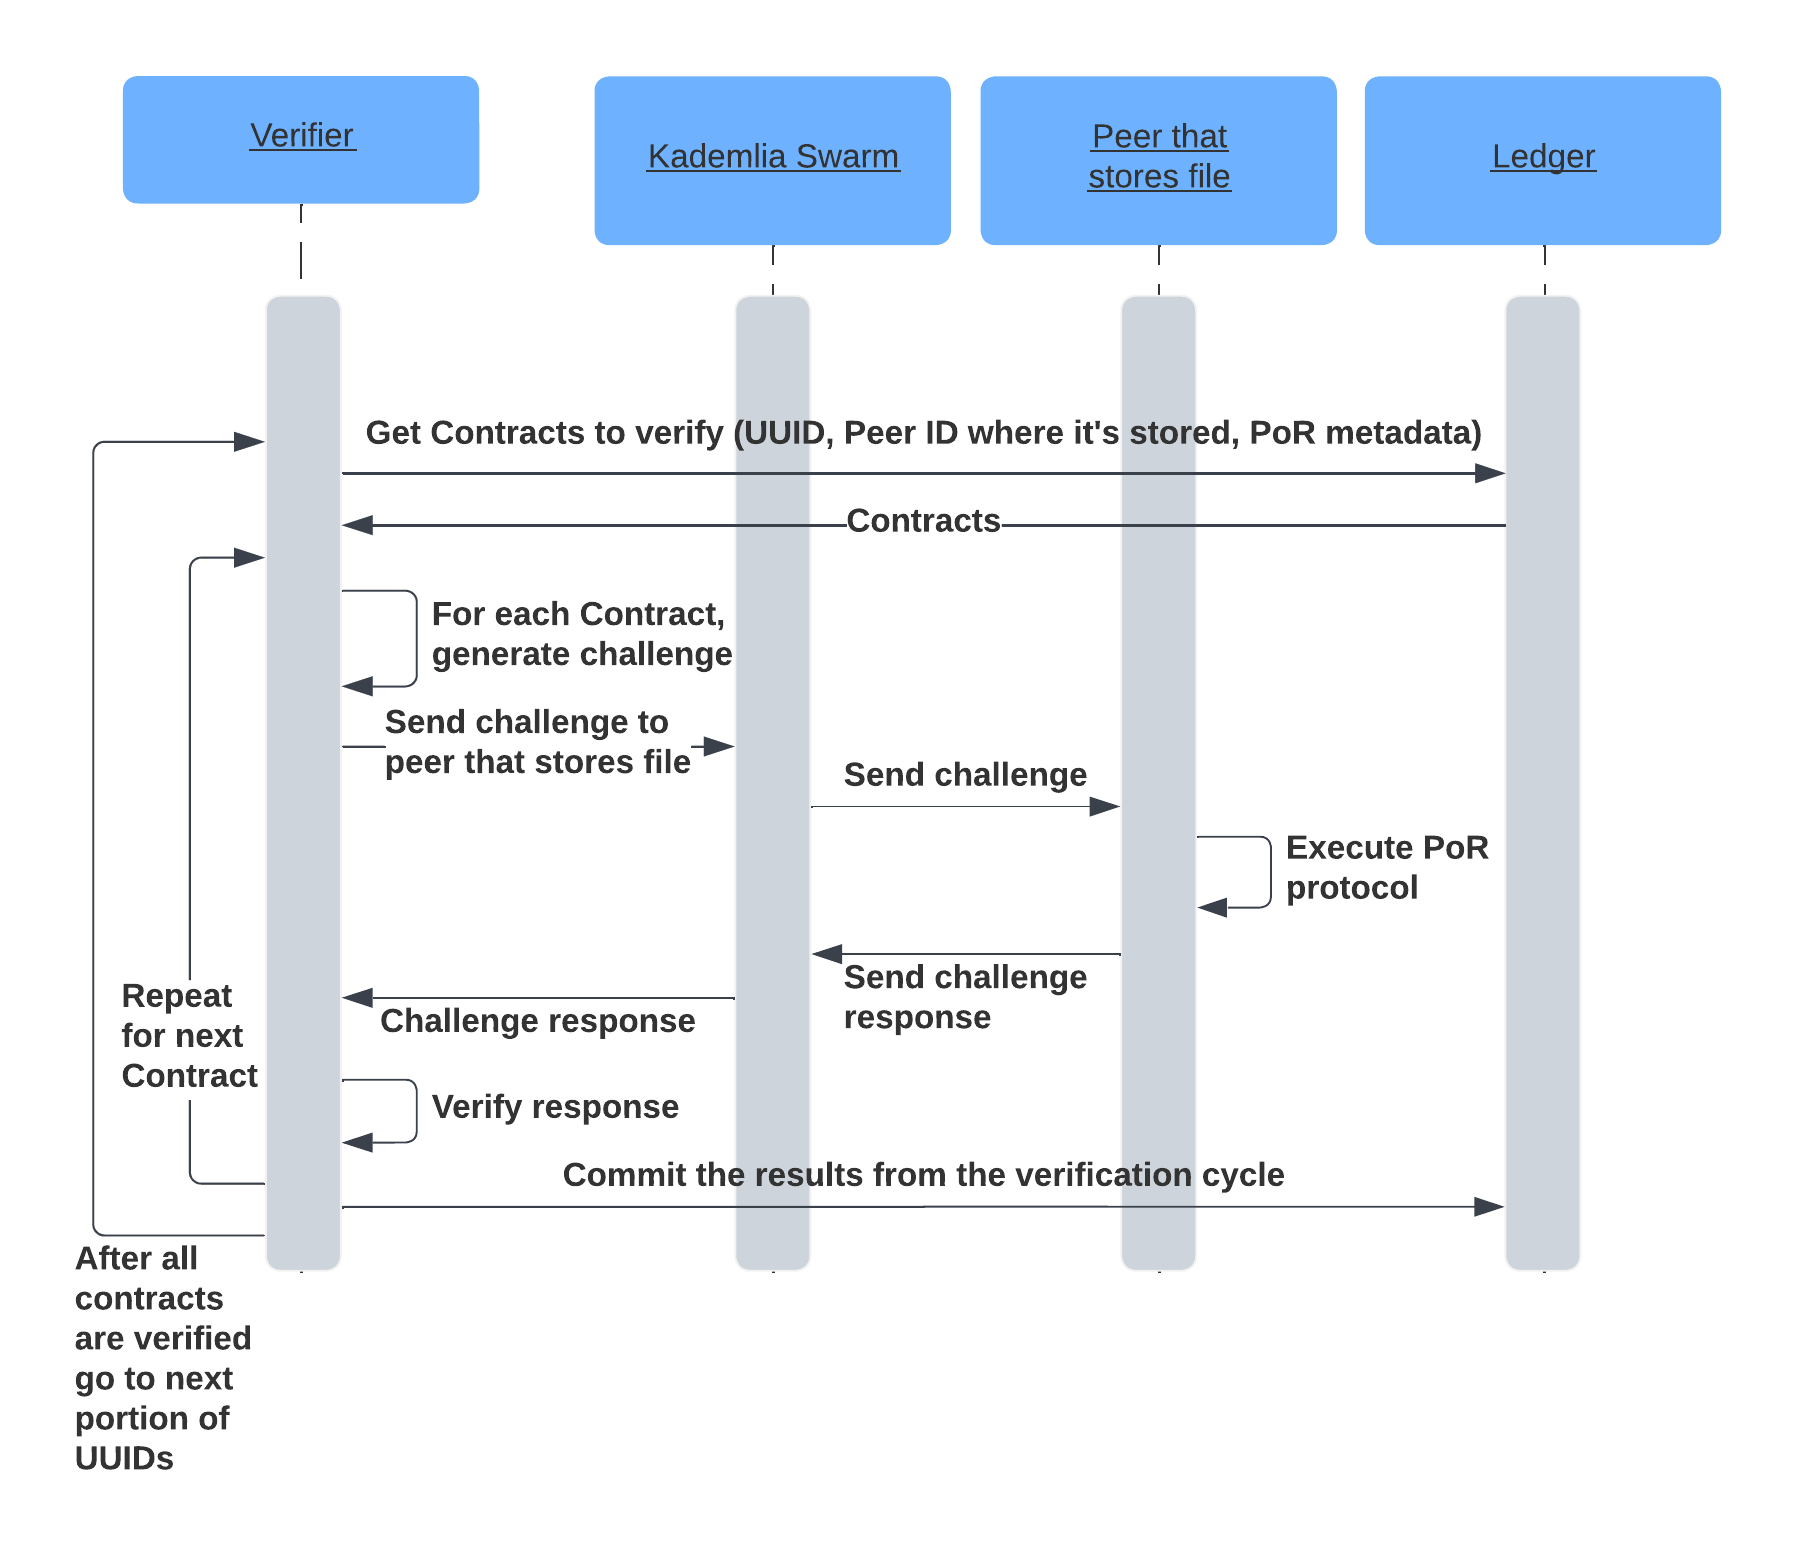
\includegraphics[width=1\textwidth]{gfx/verify.png}
    \caption{Verification of a file in the network using PoR}
    \label{fig:verify}
\end{figure}

The Proof of Retrievability (PoR) is the protocol that we use to verify that the file is stored on the peer.
The protocol is based on Dynamic proofs of retrievability with low server storage \cite{poralgebra}.
The original protocol is implemented in C and was implemented to provide an example that the protocol works.
We have implemented the protocol in Rust, and we have made some changes to the protocol to fit our use case.

The original protocol has two versions --- the default one that we are implementing, and a public version.
The public allows any peer to verify that the file is stored properly without knowing the secret vector.
For a decentralized system where we expect malicious peers, the public version is ideal,
because we do not need to worry about the malicious peers knowing the secret vector,
that is usually required to verify the file.
We have opted to not implement the public version of the protocol,
because of increased complexity, and it is not necessary to answer our research questions.

We are reusing the constants from the original protocol,
such as the prime number and chunk size.
The prime number is used for modulo arithmetic, and the authors of the paper have proven
that the protocol is secure for the given prime number.
The chunk size follows directly from the prime number size, which has 57 bits.
Since we use the prime to do modulo arithmetic, the numbers we want to work with
should be smaller.
Since computers work with bytes, which are 8 bits, we have chosen the chunk size to be 7 bytes.
Ideally we would want the chunk size to be 8 bytes, i.e., 64 bits, but this would require a prime number
with more than 64 bits, which would make the calculations slower.
Not all processors support 128-bit numbers.

Working with 7 bytes is not ideal, as we have to read the files in chunks of 7 bytes,
and then pad the last chunk with zeros before converting the chunk to a number.
We have implemented the reading of chunks in a Rust way using iterators,
which differs from the C implementation, where the language allows reading the memory directly in
chunks of 7 bytes.
The computations themselves (matrix multiplication) we have not changed,
because we wanted to test our implementation directly against the original implementation.
Apart from end-to-end tests, we wanted to test the intermediate steps of the protocol
to ensure correctness.
This is mainly because Rust does not allow direct memory manipulation and implicit type conversions,
which the C language does.

The last thing to mention is the random number generator used in the protocol.
A random number generator is used to generate the secret vector that the Keeper does not know
and the challenges for the Keeper later on.
For the purposes of testing we are using a seeded Mersenne Twister, which allows us reproducible results.
In a real-world scenario, we would use a cryptographically secure random number generator
such as ChaCha20 \cite{chacha}.
For the purposes of this thesis, a seeded Mersenne Twister is sufficient,
as it is predictable, and we do not want to test the random number generator.

\section{Reputation System}
\label{section:reputation-system}

Adding a reputation system to keep track of previous performance of the peers is essential.
It changes the way we perform the storage and verification of files,
since we need to keep track of the reputation of the peers.
The changes are reflected in \autoref{fig:store-reputation} and \autoref{fig:audit-reputation}.

\begin{figure}
    \centering
    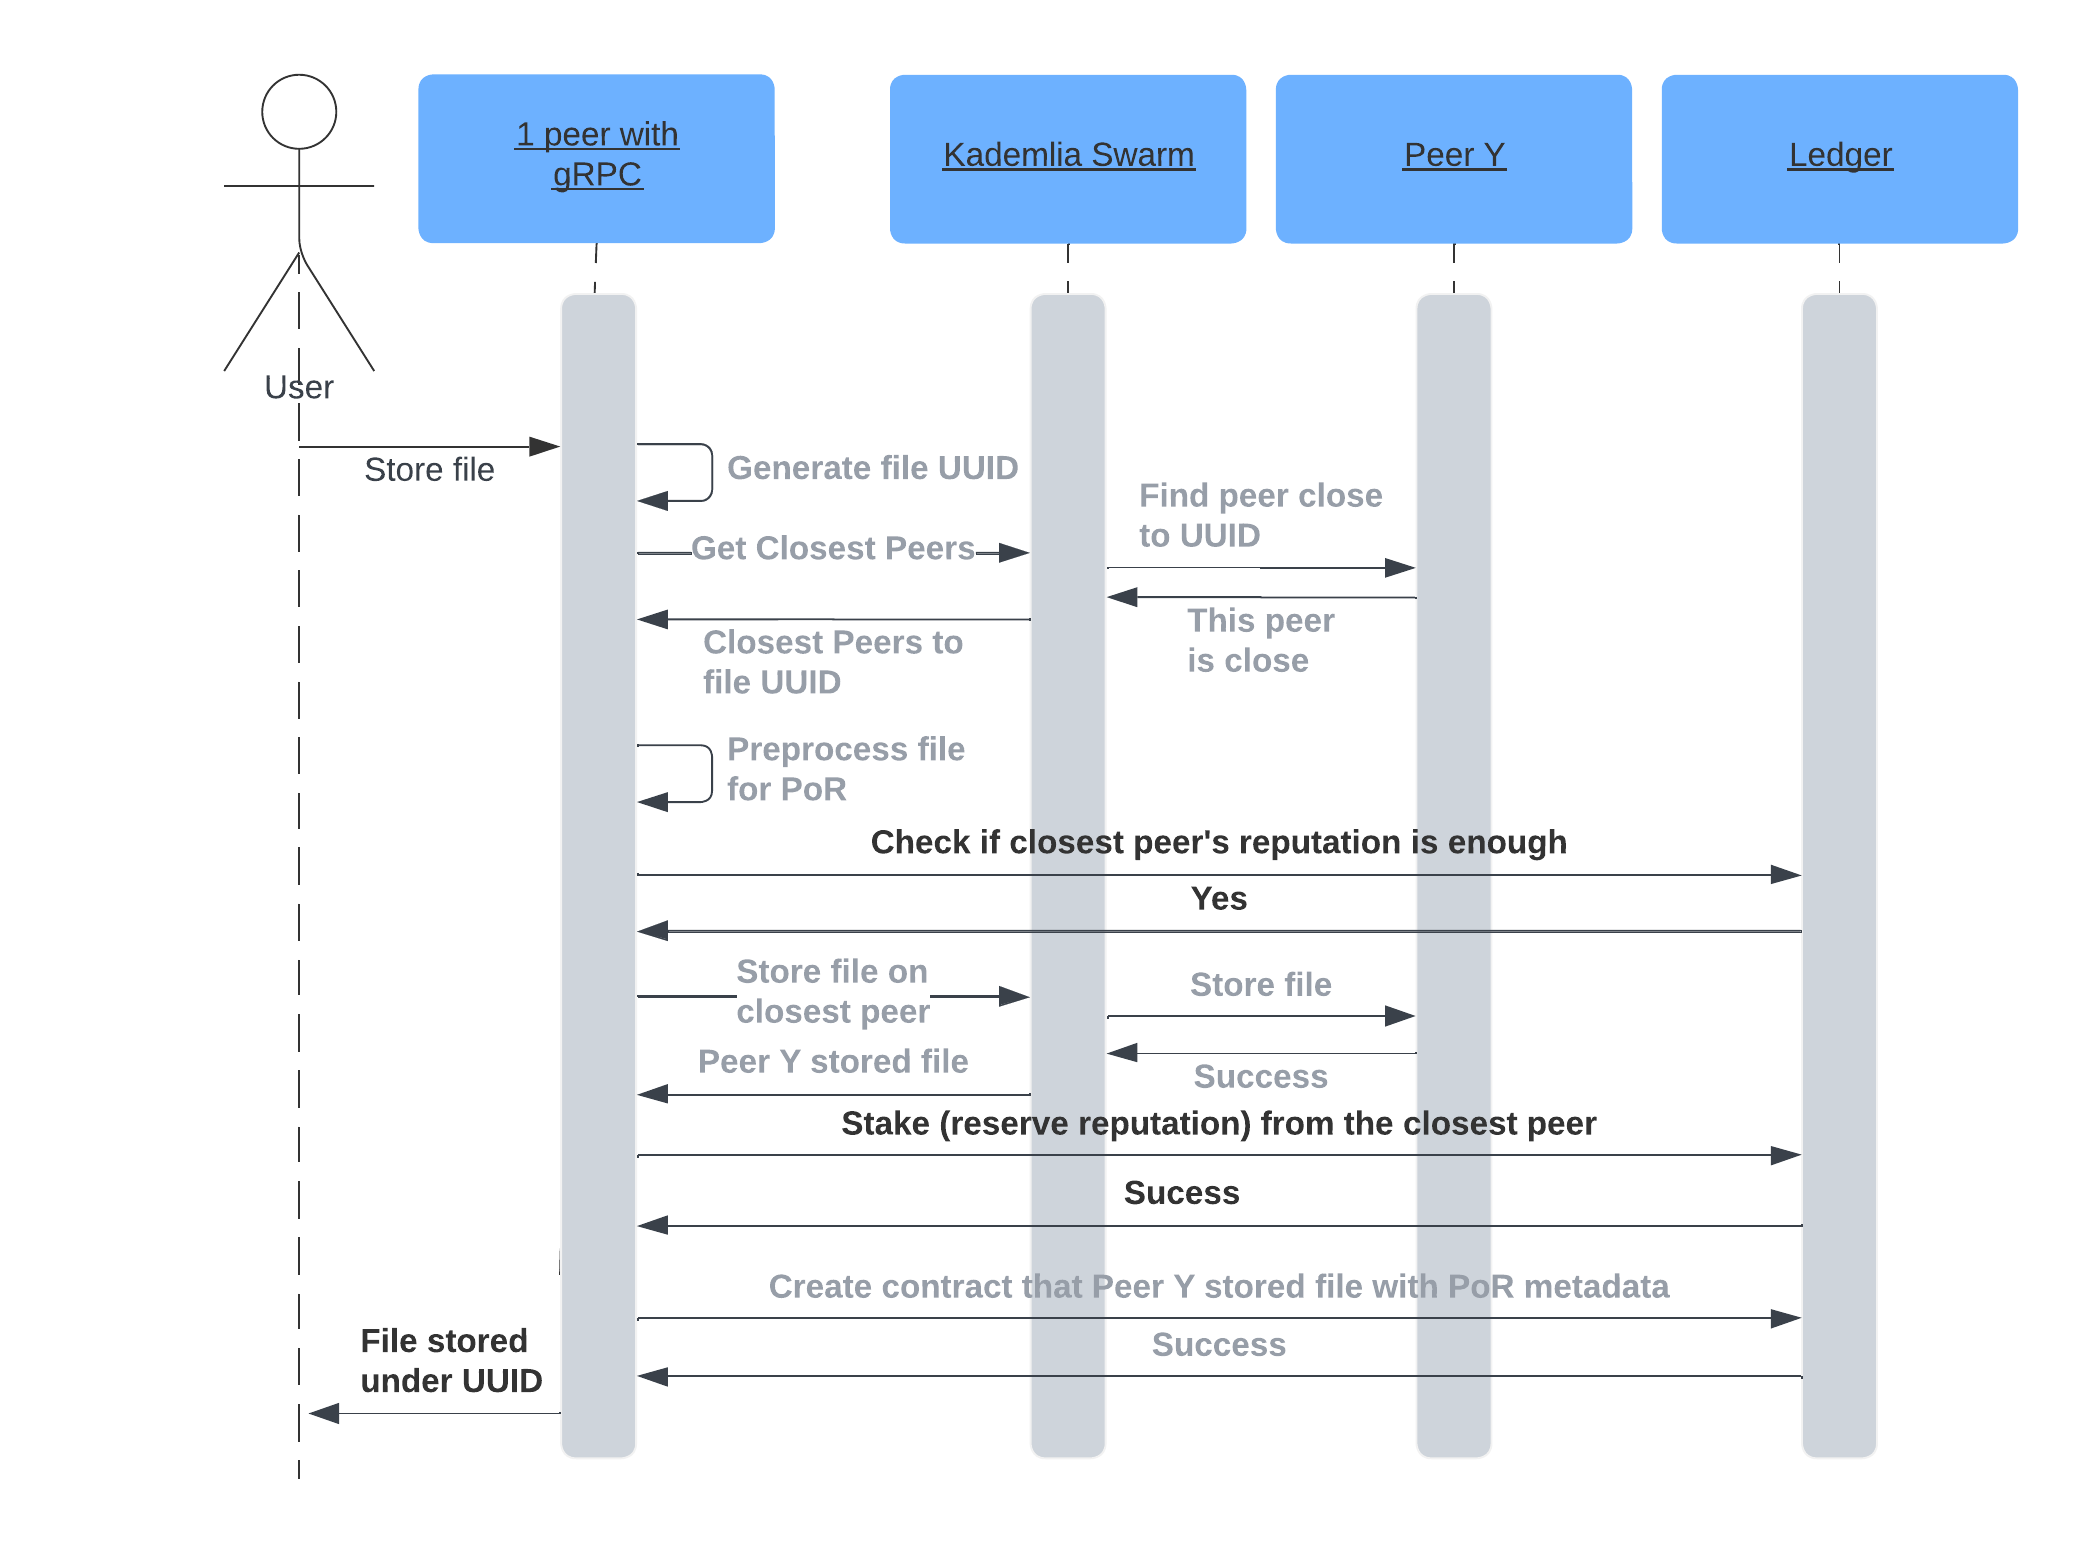
\includegraphics[width=1\textwidth]{gfx/store-reputation.png}
    \caption{Storing a new file timeline with the reputation system in place}
    \label{fig:store-reputation}
\end{figure}

\begin{figure}
    \centering
    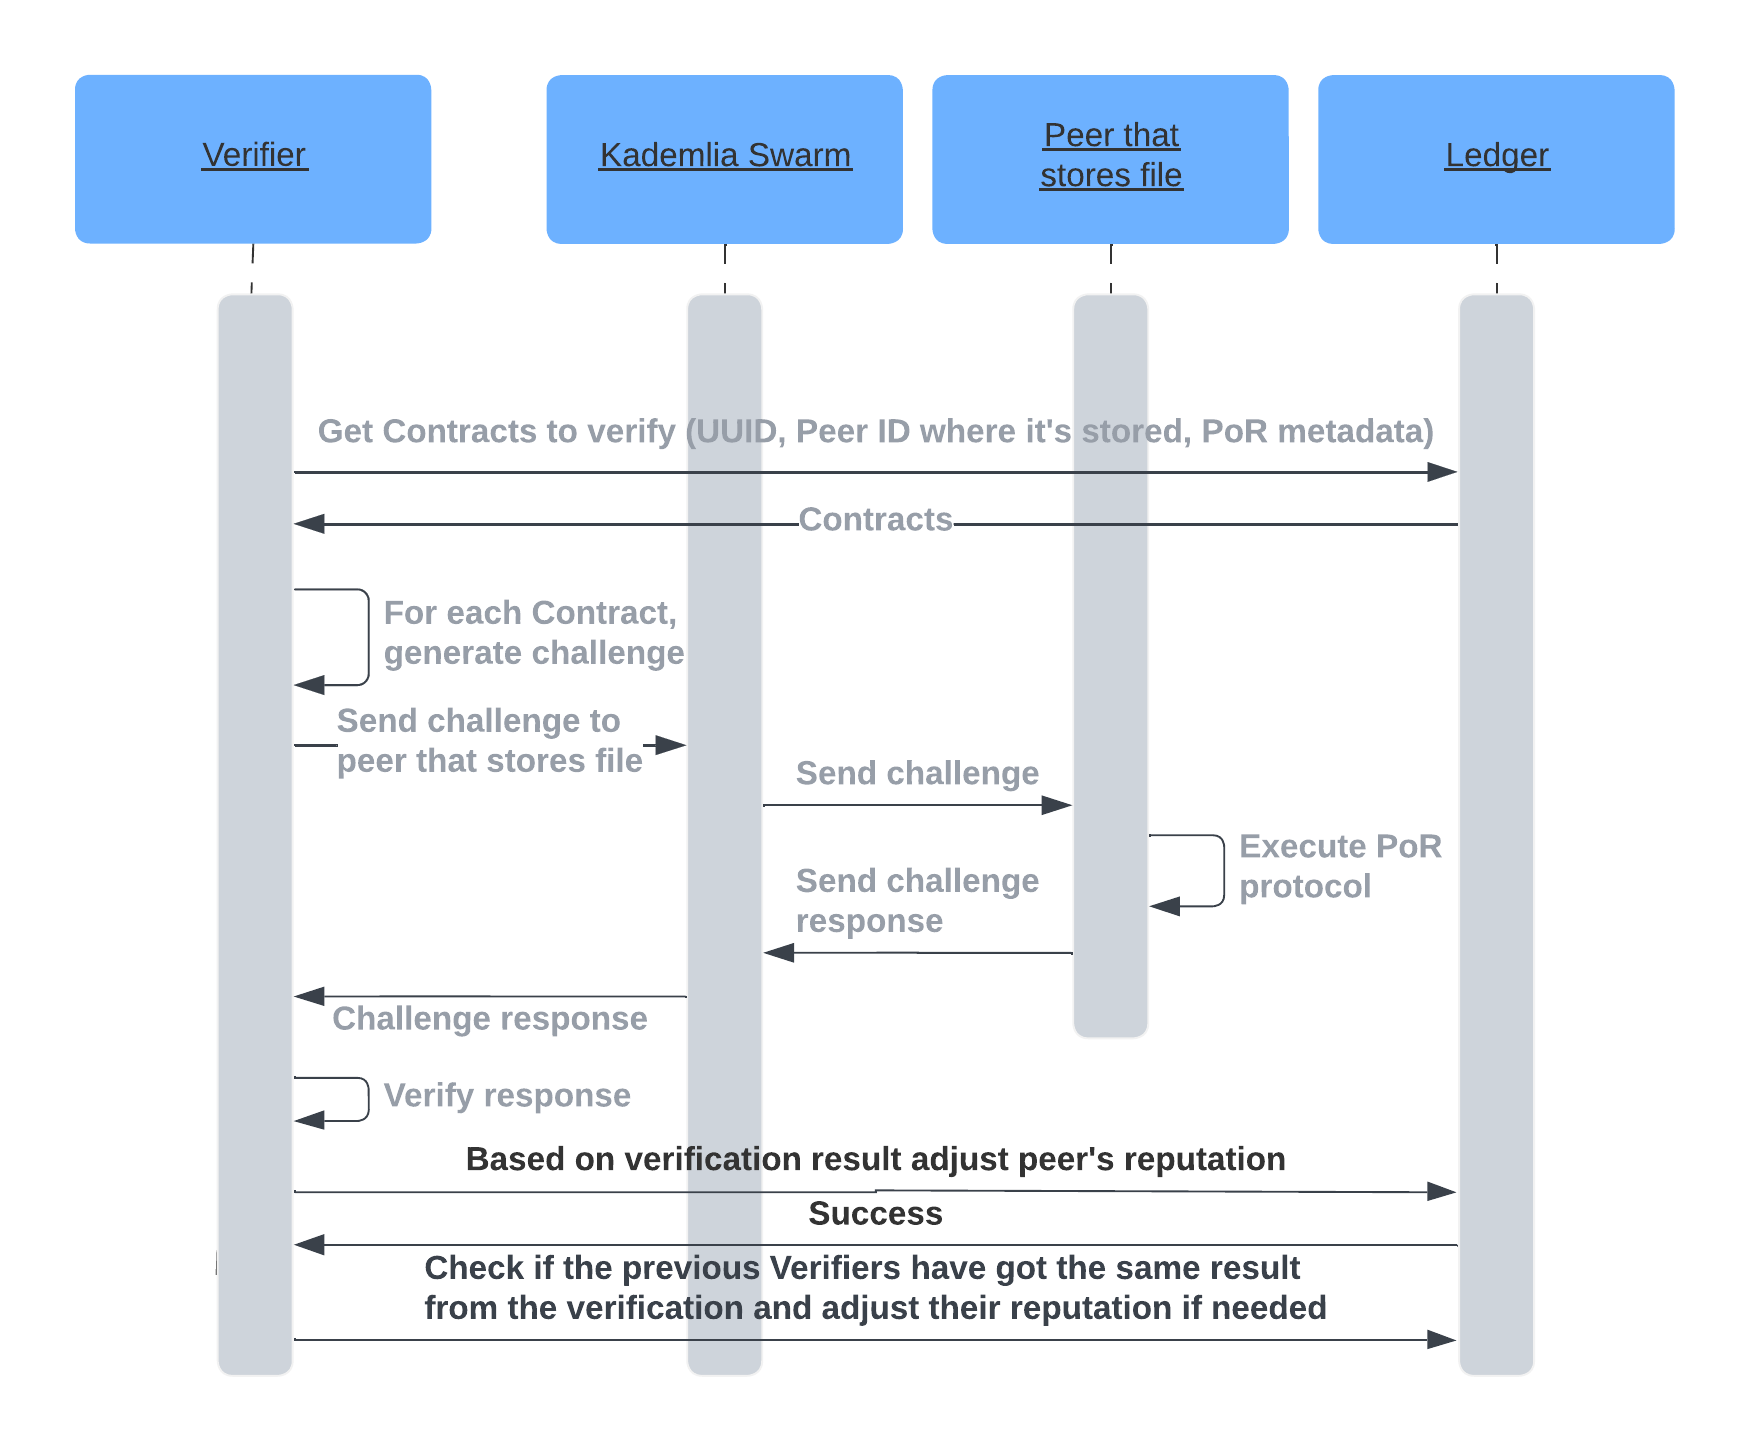
\includegraphics[width=1\textwidth]{gfx/verify-reputation.png}
    \caption{Auditing timeline with the reputation system in place}
    \label{fig:audit-reputation}
\end{figure}

Using proof of retrievability we can verify that the file is stored on a peer.
This verification happens at a fixed point in time,
and it does not guarantee that the file will be stored on the peer in the future.
It also gives us no information if the file was stored on the peer in the past.
Knowing the past performance of a peer is essential for a decentralized system,
where we know nothing else about the peers in the network.
In \autoref{chapter:analysis} we discussed how a reputation system can help us keep track
of the behavior of the peers in the network.
Ideally this reputation needs to be stored in a decentralized manner as well,
so that no peer can tamper with the reputation of another peer.

Ideally, we could use a blockchain, which is exactly a decentralized ledger,
to store the reputation of the peers.
Alternatively, we could come up with a way to store the reputation in the system itself,
since it is designed to be decentralized and aims to ensure the integrity of the data,
i.e., it should be tamper-proof.

Both of these solutions are viable for a production-ready system,
however they introduce additional complexity and potential weak points in the system,
which we have not analyzed.

For the purpose of this thesis we have decided to use the immutable database Immudb \cite{immudb}
to store the reputation of the peers.
It is centralized, but allows us to abstract ourselves from solving the problem of designing a
decentralized and tamper-proof reputation system, which is outside the scope of this thesis.
We consider the database as a single source of truth for the reputation of the peers during our tests.

The reputation system is designed to keep track of the behavior of the peers in the network.
When a peer accepts to store a file, it stakes a certain amount of reputation points.
Staking is temporary decrease of reputation points,
which is returned to the peer after the expiry date of the file.
An alternative approach is to return the reputation points to the peer in small increments
after every successful audit.

Altering the reputation is a two-step process, because we need to ensure that the operation is atomic
and Immudb does not support complex queries.
We instantiate a transaction, read the current reputation of the peer, alter it, and write it back to the database.
We go into detail about the atomic operations in \autoref{section:atomic-operations}.

Immudb provides very nice guarantees about the integrity of the data,
and we can be sure that the reputation of the peers is not tampered with.
Therefore, it is a good fit for the reputation system.
However, when we wanted to avoid the complexity of integrating with a blockchain,
we did not expect that Immudb would not support atomic operations,
and the complexity this would introduce in the system.
